\documentclass[tikz,border=10pt]{standalone}
\usepackage{amsmath}
\usetikzlibrary{calc,angles,quotes}
\begin{document}
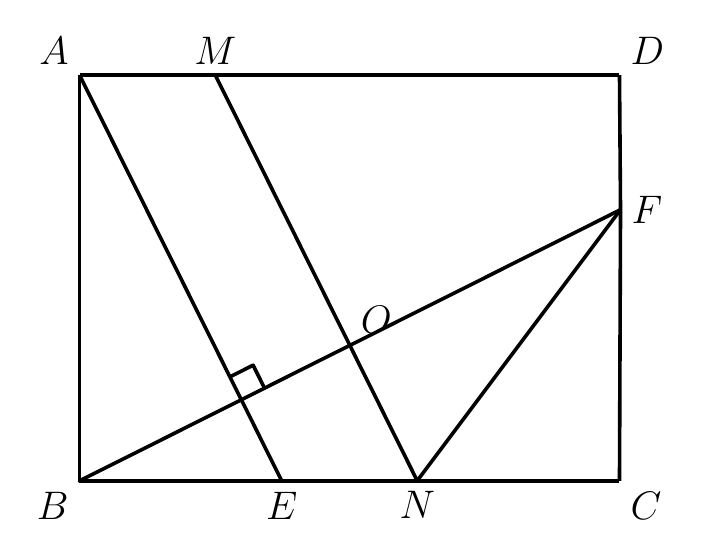
\begin{tikzpicture}[line width=1.3pt, line join=round]
\coordinate (A) at (-3.456,2.585);
\coordinate (B) at (-3.456,-2.567);
\coordinate (C) at (3.401,-2.567);
\coordinate (D) at (3.401,2.585);
\coordinate (F) at (3.414,0.876);
\coordinate (M) at (-1.732,2.585);
\coordinate (N) at (0.832,-2.566);
\coordinate (O) at (-0.025,-0.842);




\coordinate (E) at (-0.889,-2.567);
\coordinate (P) at ($(A)!(B)!(E)$);


\draw (A)--(M)--(D);

\draw (D)--(F)--(C);

\draw (C)--(B)--(A);


\draw (A)--(E);
\draw (M)--(N);
\draw (B)--(F);
\draw (F)--(N);


\draw pic[draw, angle radius=0.330cm] {right angle=A--P--F};


\node[above left, font=\fontsize{14.5}{17.4}\selectfont] at (A) {$A$};
\node[above, font=\fontsize{14.5}{17.4}\selectfont] at (M) {$M$};
\node[above right, font=\fontsize{14.5}{17.4}\selectfont] at (D) {$D$};
\node[right, font=\fontsize{14.5}{17.4}\selectfont] at (F) {$F$};
\node[above right, font=\fontsize{14.5}{17.4}\selectfont] at (O) {$O$};
\node[below right, font=\fontsize{14.5}{17.4}\selectfont] at (C) {$C$};
\node[below left, font=\fontsize{14.5}{17.4}\selectfont] at (B) {$B$};
\node[below, font=\fontsize{14.5}{17.4}\selectfont] at (E) {$E$};
\node[below, font=\fontsize{14.5}{17.4}\selectfont] at (N) {$N$};
\end{tikzpicture}
\end{document}